\documentclass[11pt, letterpaper]{article}
\usepackage[utf8]{inputenc}
\usepackage{graphicx}
\graphicspath{{images/}}
\usepackage{amsmath}
\usepackage{amssymb}
\usepackage{fancyhdr}

\pagestyle{fancy}
\fancyhf{}
\rhead{ECE 316}
\lhead{Spring 2017}
\rfoot{\thepage}
\title{ECE316 Lecture Note 1 by Prof. Xie - Spring 2017}
\author{Prof. Liang-Liang Xie}
\date{\today}

\begin{document}
\section{Combinational Analysis}
\subsection{Introduction}
\textbf{Example}: A communication system consists of 4 antennas

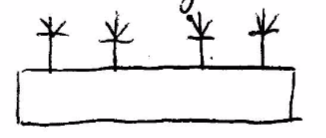
\includegraphics{1-1}

Assume that this system will be functional if no two consecutive antennas are defective. \newline \newline
\noindent
\underline{Q:} If there are exactly 2 antennas defective, what is the probability that the resulting system will be functional? \newline \newline
\noindent
\underline{Solution:}
\begin{center}
  \begin{tabular}{ c c c c c c }
    0 1 1 0 & 0 1 0 1 & 1 0 1 0 & 0 0 1 1 & 1 0 0 1 & 1 1 0 0 \\
    $\surd$ & $\surd$ & $\surd$ & $\times$ & $\times$ & $\times$
  \end{tabular}
\end{center}

If all the cases are equally likely, the probability is \( \frac{3}{6} \)=\( \frac{1}{2} \).

\subsection{The Basic Principle of Counting}
Suppose that two experiments are to be performed. If experiment 1 can result in any one of $m$ possible outcomes, and if for each outcome of experiment 1, there are $n$ possible outcomes of experiment 2, then together there are $m \times n$ possible outcomes of the two experiments.
\begin{center}
  \begin{tabular}{ c c c c }
    (1,1) & (1,2) & \dots & (1,n) \\
    (2,1) & (2,2) & \dots & (2,n) \\
    $\vdots$ & $\vdots$ & $\ddots$ & $\vdots$ \\
    (n,1) & (n,2) & \dots & (n,m)
  \end{tabular}
\end{center}
\textbf{Example}: A small community, 10 women, each has 3 children. If one women and one of her children are to be selected as mother and child of the year. How many possibilities? \newline
\noindent
\underline{Solution:} $10\times3 = 30$ \newline

\noindent\underline{Generalize:} \newline
Experiment 1 with $n_1$, possible outcomes, for each of them. There are $n_2$ outcomes of experiment 2, for each of them. There are $n_3$ possible outcomes of experiment 3\dots\dots then there are totally, \newline
\begin{equation*}
  n_1 \cdot n_2 \cdot n_3 \dots n_r
\end{equation*}
possible outfcomes of the r experiments. \newline \newline
\noindent
\textbf{Example}: How many different 7-place license plates are possible if the first 3 places are to be occupied by letters and the final 4 by numbers? \newline \newline
\noindent
\underline{Solution:}
\begin{equation*}
  26 \times 26 \times 26 \times 10 \times 10 \times 10 \times 10 = 175,760,000
\end{equation*}
\underline{Q:} What if repetition among letters or numbers are prohibited? \newline \newline
\underline{Solution:}
\begin{equation*}
  26 \times 25 \times 24 \times 10 \times 9 \times 8 \times 7 = 78,624,000
\end{equation*}

\subsection{Permutations}
\textbf{Example}: How many different ordered arrangements of $a, b, c$? \newline \newline
\noindent
\underline{Solution:}
\begin{equation*}
  abc; acb; bac; bca; cab; cba
\end{equation*}
Each is known as a permutation.
By the basic principle of counting:
\begin{equation*}
  3 \cdot 2 \cdot 1 = 6
\end{equation*}
\newline
\noindent
Generally, for $n$ objects, there are:
\begin{equation*}
  n \cdot (n-1) \cdot (n-2) \cdot \dots \cdot 2 \cdot 1 = n!
\end{equation*}

different permutations. \newline \newline
\noindent
\textbf{Example}: To put 10 books on the bookshelf. Of these, 4 are math, 3 are chemistry, 2 are history, 1 is language. The books of the same subject should be put together. How many different arrangements? \newline \newline
\noindent
\underline{Solution:}
\begin{multline*}
  4! \cdot 3! \cdot 2! \cdot 1! \cdot 4! = 6912 \\
  (10!\text{ without the restriction that the books of the same subject should be put together})
\end{multline*}
\textbf{Example}: A class consists of 6 men and 4 women. An exam is given an no two students obtain the same score.

(a) How many different rankings are possible?
\begin{equation*}
  10! = 3,6628,800
\end{equation*}

(b) If men and women are ranked separately, how many?
\begin{equation*}
  4! \cdot 6! = 17,280
\end{equation*} \\ \\
\noindent
\textbf{Example}: How many different letter arrangements can be formed using the letters $PEPPER$? \newline \newline
\noindent
\underline{Solution:}
\begin{equation*}
\frac{6!}{3!\cdot2!} = 60, \left.
  \begin{array}{r}
    P_1EP_2P_3ER \\
    P_2EP_1P_3ER \\
    P_3EP_2P_1ER \\
    \vdots       \\
    \vdots       \\
    P_1EP_3P_2ER
  \end{array} \right\} 3! \text{ arrangements}
\end{equation*}
\newline \noindent
In general, there are
\begin{equation*}
  \frac{n!}{
    n_1!\cdot n_2!\cdot n_3!\cdot \dots n_r!
  },  (n = n_1 + n_2 + n_3 + \dots + n_r)
\end{equation*}
diffierent permutations of $n$ objects, of which $n_1$ are alike, $n_2$, $n_3$ are alike, \dots , $n_r$ are alike. \newline \newline
\noindent
\textbf{Example}: How many different signals, by hanging 9 flags in a line, 4 white, 3 red, 2 blue? \newline \newline
\noindent
\underline{Solution:}
\begin{equation*}
  \frac{9!}{4! \cdot 3! \cdot 2!} = 1260
\end{equation*} \\ \\
\subsection{Combinations}
First, a \textit{question}: How many different groups of 3 can be selected from the 5 items $A,B,C,D,E$?
\begin{align*}
  &\frac{5 \times 4 \times 3}{3!} = 10 \\
  (\text{Hint:} \{AB&C\}, \{ACB\}, \dots \{BAC\} \text{are the same group}.)
\end{align*} \\
In general, selecting $r$ items from $n$ items, then the number of different groups is
\begin{align*}
  &\quad   \frac{n(n-1)(n-2)\dots(n-r+1)}{r!} \\
  & = \frac{n!}{(n-r)!\cdot r!} \\
  & = \binom{n}{r} \\
\end{align*}
\begin{equation*}
  \binom{n}{n} = 1, \hspace{1cm} \binom{n}{1} = n, \hspace{1cm} \binom{n}{0} = 1 = \frac{n!}{n!\cdot 0!}, (0! = 1 \text{ by convention})
\end{equation*} \\ \\
\noindent
\textbf{Example}: From 5 women and 7 men, how many different committees of 2 women and 3 men can be formed? \\ \\
\noindent
\underline{Solution:}
\begin{equation*}
  \binom{5}{2} \cdot \binom{7}{3} = \frac{5\cdot 4}{2\cdot 1}\cdot \frac{7\cdot 6\cdot 5}{3\cdot 2\cdot 1} = 350
\end{equation*}
\underline{Q:} What if 2 of the men refuse to serve together?
Suppose the 2 men are $A$ and $B$, then there are 4 situations:
\begin{enumerate}
  \item both A and B are in $\binom{5}{2}\cdot \binom{5}{1}$
  \item A in, B out $\binom{5}{2}\cdot \binom{5}{2}$
  \item A out, B in $\binom{5}{2}\cdot \binom{5}{2}$
  \item neither is in $\binom{5}{2}\cdot \binom{5}{3}$
\end{enumerate}
So the answer is $350 - \binom{5}{2}\binom{5}{1}$ \\
(Alternative answer is $\binom{5}{2}\binom{5}{2}\cdot 2 + \binom{5}{2}\binom{5}{3}$ or $\frac{\binom{5}{2}\binom{6}{3}}{2} + \frac{\binom{5}{2}\binom{6}{3}}{2} \times 2$ \\ \\

\noindent
\textbf{Example}: $n$ antennas with $m$ defective \\
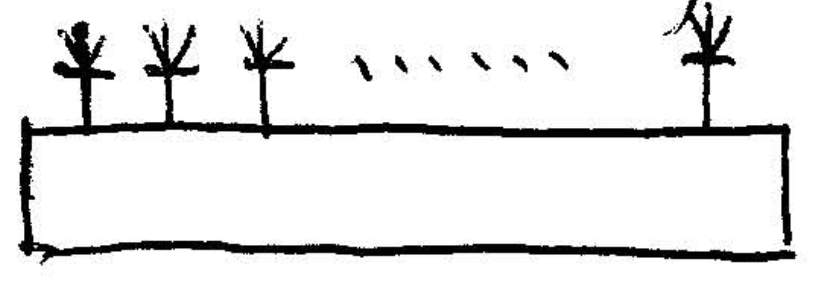
\includegraphics{1-2} \\
The system will be function if no two consecutive ones are defective. What is the probability of being funtional? \\ \\
Hint: There are two steps to consider the problem:
\begin{enumerate}
  \item Totally, how many possibilities of finding $m$ defective in $n$? ($M$)
  \item Among them, how many where no two consecutive is defective? ($N$)
\end{enumerate}
The probability should be $\frac{M}{N}$. \\ \\
\underline{Solution:}
\begin{enumerate}
  \item The total number of possibilities: $\binom{n}{m}$
  \item The total number of cases where no two consecutive ones: $\binom{n-m+1}{m}$
\end{enumerate}
Hint: $n-m$ working ones in a line give rise to $n-m+1$ holes. \\

\includegraphics{1-3} \\
Each hole can contain at most one defective antenna, so it is required to choose $m$ holes from the $n-m+1$ holes to place defective antennas. \\ \\
So, the probability of being functional is $\frac{\binom{n-m+1}{m}}{\binom{n}{m}}$. where of $n-m+1 = m$, the probability is 0. \\ \\

\noindent
A useful combinational identity is $\binom{n}{r} = \binom{n-1}{r-1} + \binom{n-1}{r}$ \\ \\
\textit{Proof:}
\begin{align*}
  \binom{n-1}{r-1} + \binom{n-1}{r} &= \frac{(n-1)!}{(r-1)!(n-r)!} + \frac{(n-1)!}{r!(n-1-r)!} \\
  &= \frac{(n-1)!r}{(n-r)! r!} + \frac{(n-1)!(n-r)}{r!(n-r)!} \\
  &= \frac{(n-1)!(n-r+r)}{(n-r)!r!} \\
  &= \frac{n!}{(n-r)!r!} = \binom{n}{r}
\end{align*} \\ \\

\noindent
\textit{Combinational Argument}: Suppose there are $n$ items, then $\binom{n}{r}$ is the number of different ways to choose $r$ items from the $n$ items. Besides, we con consider the first item, which can be chosen or not. if the 1st is chosen, then we only have to choose $r-1$ from the $n-1$ items, which gives rise to the $\text{number} - \binom{n-1}{r-1}$. If we don't choose the 1st, then there are $\binom{n-1}{r}$ ways to choose $r$ from the $n-1$ items. Combining the above two cases, it follows:
\begin{equation*}
  \binom{n}{r} = \binom{n-1}{r-1} + \binom{n-1}{r}
\end{equation*} \clearpage

\noindent
The binomial thorem:
\begin{align*}
  (x+y)^n &= \sum_{k=0}^n \binom{n}{k} \cdot x^k \cdot y^{n-k} \hspace{1.0cm} (\binom{n}{k} \text{ terms of } x^k y^{n-k}) \\
  &= \sum_{k=0}^n \binom{n}{n-k} \cdot x^k \cdot y^{n-k} \hspace{0.3cm} (\binom{n}{n-k} \text{ terms of } x^k y^{n-k}) \\
  \text{Obviously, } &\binom{n}{k} = \binom{n}{n-k}, \text{ since } \binom{n}{k} = \frac{n!}{(n-k)!k!} = \binom{n}{n-k}.
\end{align*} \\
For mathematical proof of the theorem, please see the textbook. \\ \\
\noindent
\textbf{Example}: $(x+y)^3 = x^3 + 3x^2y + 3xy^2 + y^3$ \\ \\
\noindent
\textbf{Example}: How many subsets are there of a set consisting of $n$ elements?
\begin{equation*}
  \{1,2,3, \dots n\}
\end{equation*}
\noindent
\underline{Solution:}
\begin{equation*}
  \begin{array}{l}
    \varnothing, \{1\}, \{2\}, \{3\} \dots \{n\}; \\
    \{1,2\}, \{1,3\} \dots \{n, n-1\}; \\
    \vdots \\
    \{1,2,3 \dots n\}
  \end{array}
\end{equation*} \\
\begin{center}
$\Downarrow$ \\
\end{center}
\begin{equation*}
  \binom{n}{0} + \binom{n}{1} + \binom{n}{2} + \binom{n}{3} + \dots \binom{n}{n} = \sum_{k=0}^n \binom{n}{k} = ? \hspace{0.5cm} (2^n)
\end{equation*} \\
Applying the binomial theorem and letting $x$ and $y$ being 1s, then
\begin{equation*}
  \sum_{k=0}^n \binom{n}{k} = \sum_{k=0}^n \binom{n}{k}\cdot1^k\cdot1^{n-k} = (1+1)^n = 2^n
\end{equation*} \\
Besides, we can consider this problem in another way: Forming a subset from the set consisting of $n$ elements can be regarded as choosing some elements from that set. So, for each element, it has two choices, whether to be chosen to form the subset or not.
\begin{align*}
  \{1, 2, &3, 4\dots n\} \\
  &\downarrow \\
  &\text{each of them could be chosen for subset or not.}
\end{align*} \\
Thus, by the basic principle of counting, there are $2^n$ subsets. \\ \\
\subsection{Multinomial Coefficients}
\underline{Q:} $n$ distinct items are to be divided into $r$ distinct groups of respective sizes $n_1, n_2, \dots n_r\quad(n_1 + n_2 + n_3 + \dots + n_r = n)$. How many different divisions are possible? \\ \\
\noindent
To fill the $r$ groups step by step, we not that there are $\binom{n}{n_1}$ possible choices for the first group, $\binom{n-n_1}{n_2}$ possible choices for the second group, \dots and $\binom{n-n_1-n_2\dots-n_{r-1}}{n_r}$ choices for the $r$th group. Thus, it follows from the generalized version of basic principle of counting that there are
\begin{align*}
  &\binom{n}{n_1}\binom{n-n_1}{n_2}\binom{n-n_1-n_2}{n_3}\dots\binom{n-n_1-n_2\dots-n_{r-1}}{n_r} \\
  = &\frac{n!}{(n-n_1)!n_1!}\cdot\frac{(n-n_1)!}{(n-n_1-n_2)!n_2!}\cdot\frac{(n-n_1-n_2)!}{(n-n_1-n_2-n_3)!n_3!}\dots\frac{n-n_1-n_2\dots-n_{r-1}}{0!n_r!} \\
  = &\frac{n!}{n_1!n_2!n_3!\dots n_r!} \text{ possible divisions}.
\end{align*} \\
(Can the answer be $r^n$? No! Consider the specific situation where $n_1 = 1$, for the first item there are $r$ choices, but for the second item, the number of possible choices will depend and may not be $r$ any longer) \clearpage
\textit{Alternative reasoning:} We can change the problem to how to throw $n$ items into $n$ holes as the following figure: \\
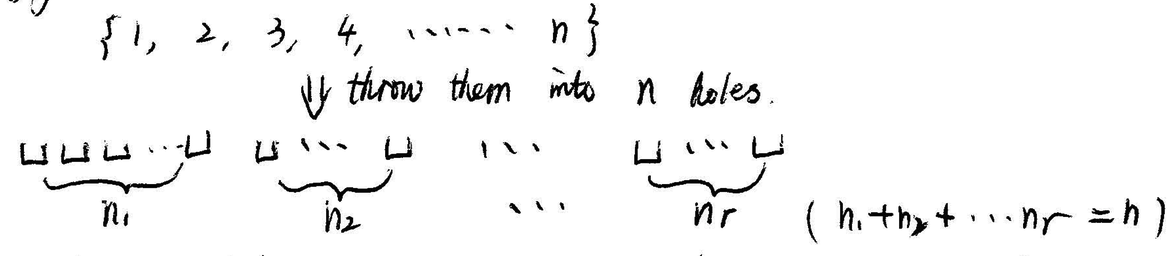
\includegraphics[scale=0.25]{1-4} \\
Each permutation can be regarded as a way to group them, but if we take $n!$ as the total number of possible ways to group them, we have over counted, because it doesn't matter how we permute the items in the same group among themselves. \\
Thus, there are $\frac{n!}{n_1!n_2!\dots n_r!}$ possible divisions. \\ \\
\noindent
Still, we can take this problem as how to assign $n$ labels to $n$ items. Of the $n$ labels, $n_1$ are alike, $n_2$ are alike, \dots $n_r$ are alike. If one item receives the $k$-th  label, then it's contained by the $k$-th group. \\
\vspace{0.2cm}


\includegraphics[scale=0.7]{1-5} \\

\vspace{0.2cm}

Notation: \begin{equation*}\frac{n!}{n_1!n_2!\dots n_r!} = \binom{n}{n_1,n_2,\dots n_r}\end{equation*} \\ \\
\noindent
\textbf{Example:} 10 children are to be divided into 2 basketball teams, each of 5 to play against each other, how many different divisions? \\
\begin{equation*}
  \frac{\frac{10!}{5!5!}}{2}, \text{(There is a 2 in the denominator because the order of the two teams is irrelevant.)}
\end{equation*} \\
Recall the binomial theorem, which is \begin{equation*}
  (x+y)^n = \sum_{k=0}^n \binom{n}{k} x^k \cdot y^{n-k}
\end{equation*} \\
Accordingly, the multinomial theorem is \begin{equation*}
  (x_1+x_2+\dots x_r)^n = \sum_{n_1+n_2+\dots n_r = n}\binom{n}{n_1,n_2,\dots n_r}x_1^{n_1} x_2^{n_2} \dots x_r^{n_r}
\end{equation*}

\end{document}
